% Modelling with identification and Hysteresis consideration

\chapter{Modelling of McKibben Artificial Muscles}

In this Chapter, the muscle models used as nominal models for model-based control are derived.

\section{Introduction}

McKibben muscles are actuators used mainly for medical purposes in rehabilitation and welfare. 
The reason is their high flexibility, light weight, low cost, human and environmental friendliness and ease of use.
As mentioned in Chapter~\ref{ch:introduction}, the control of this kind of actuators
is often problematic, due to their inherent high nonlinearity.

Many muscle models have been proposed, both static and dynamic.
One of the most known static models is derived by Chou~\cite{model_chou},
which is based on the equilibrium between the input pressure and the release of energy.
Although the main interest is to obtain the dynamic model to use in control, 
the static one is also reviewed and evaluated because they are used with feed-forward
control applied to rehabilitation devices using the McKibben muscle. 

Dynamic muscle models can be categorized in analysis oriented and control oriented.
Analysis oriented models provide very high accuracy, but they are also very complex.
For this reason they are not much suitable for control purposes.

Control oriented models provide lower accuracy than analysis oriented ones,
but their lower complexity allows them to be used more efficiently for control.

%TODO: add existing research on muscle models

Since tap water driven muscles are simpler than pneumatic ones, the idea is to use
linear system identification and obtain a simple model of the muscle's dynamics.
Being this only a linear model,
it does not take into account the presence of strong nonlinearities,
such as the friction between the braids and the hysteretic behaviour of the muscle.
However, the introduction of a hysteresis model can lead to achieving higher precision
with the model derived from linear system identification.

Through history, several hysteresis models have been developed.
Notable examples are the Maxwell-slip model~\cite{al2005generalized},
the Jiles-Atheron model~\cite{lederer1999parameter}
and the Preisach model~\cite{ge1997generalized}. 
Common interest points of these models are friction of the braided sleeve,
and the hysteresis caused by it, which both add nonlinearities to the model.

These hysteresis models are precise, yet complex in structure.
To overcome this problem, the Bouc-Wen~\cite{bouc}~\cite{bouc_wen} hysteretic model is combined with 
the identified muscle model. Including the hysteretic model raises the number
of parameters that have to be identified for the system, but this is easily
achieved, at first, by trial and error. Later, an adaptive algorithm is developed
to get the best parameters for the muscle, and thus the updated model can be use
as a nominal model for model-based control techniques.

The accuracy of the proposed model is compared to experimental results
by analysing the pressure--displacement characteristics and the hysteresis characteristics.
Moreover, the effects of changing the load of the muscle are studied,
because they may have a great impact upon control performances.

\section{Static Model}


\subsection{Introduction}
The relationship between the axial contraction force and the pressure difference
amid supply and atmospheric pressure has been reported in different papers~\cite{chou1994static}~\cite{schulte}.

The association is based on the equilibrium between the input work in the McKibben muscle
(\ie~when the fluid is supplied to the inner rubber tube)
and the output work (\ie~when the actuator shortens or elongates
because of the volumetric change associated with the pressure difference).

Figure~\ref{fig:muscle_structure} shows the geometric structure,
which follows the geometric relationships in Equation~\ref{eq:geom_rel_1}.


\begin{figure}[H]
	\centering
	\begin{minipage}{.4\textwidth}
		\centering
		\begin{tikzpicture}
			\draw (0,0) arc (0:180:0.5 and 0.2);
			\draw (-1,0) -- (-1,-5);
			\draw (0,-5) -- (0,0);
			\draw[] (-0.625,0.2) -- (-0.625,0.5);
			\draw[] (-0.375,0.5) arc(0:180:0.125 and 0.05);
			\draw[densely dotted] (-0.625,0.5) arc(180:360:0.125 and 0.05);
			\draw[] (-0.375,0.5) -- (-0.375,0.2);
			\pattern[pattern=north east hatch,hatch distance=2.5mm] (-1,0) -- (-1,-5) arc(180:360:0.5 and 0.1) -- (0,0) arc (0:180:0.5 and 0.2);
			\pattern[pattern=north west hatch,hatch distance=2.5mm] (-1,0) -- (-1,-5) arc(180:360:0.5 and 0.1) -- (0,0) arc (0:180:0.5 and 0.2);
			\fill[white] (0,-5) arc(0:360:0.5 and 0.1);
			\draw (-1,-5) arc(180:255:0.5 and 0.1);
			\draw (0,-5) arc(360:285:0.5 and 0.1);
			\draw (0,-5) arc(0:180:0.5 and 0.1);
			\draw[] (-0.375,-5) arc(0:180:0.125 and 0.025);
			\draw[] (-0.625,-5) -- (-0.625,-5.3);
			\draw[] (-0.625,-5.3) arc(180:360:0.125 and 0.05);
			\draw[] (-0.375,-5.3) arc(0:180:0.125 and 0.05);
			\draw[] (-0.375,-5.3) -- (-0.375,-5);
			\node at (-1.25,0) (nA) {};
			\node at (-1.25,-5) (nB) {};
			\node[align=center] at (1.4,0.4) (tubeText) {Rubber \\ Tube};
			\node[align=center] at (1.4,-2.5) (sleeveText) {Nylon \\ Sleeve};
			\draw (-0.5,0.4) -- (tubeText);
			\draw (-0.1,-2.5) -- (sleeveText);
			\Dimline[($(nB)$)][($(nA)$)][$L$][0.25];
			\node at (-1,-5.5) (nC) {};
			\node at (0,-5.5) (nD) {};
			\Dimline[($(nC)$)][($(nD)$)][$D$][-0.25];
		\end{tikzpicture}
	\end{minipage}
	\begin{minipage}{.4\textwidth}
		\centering
		\begin{tikzpicture}
			\draw (0,0) coordinate (L) node {}
				-- (0,4) coordinate (O) node {}
				-- (2,0) coordinate (R) node {}
				pic["$\psi$", ->,draw=black, angle eccentricity=1.3, angle radius=1cm]{angle=L--O--R};
			\draw (0,-0.5) -- (0,0);
			\draw (0,0) -- (2,0);
%			\filldraw[] (0,4) circle (1pt);
			\draw[very thick] (0,4) -- (2,0);
			\draw (2,0) -- (2,-0.5);
			\node at (2,3.75) (threadText) {Thread};
			\draw (0.11,3.75) -- (threadText);
			\node at (0,-1) (nA) {};
			\node at (2,-1) (nB) {};
			\Dimline[($(nA)$)][($(nB)$)][$\pi n D$][-0.25];
			\node at (0.1,4.05) (nO) {};
			\node at (2.1,0.05) (nC) {};
			\Dimline[($(nO)$)][($(nC)$)][$b$][0.25];
		\end{tikzpicture}
	\end{minipage}
	\caption{Geometric structure of a McKibben artificial muscle}
	\label{fig:muscle_structure}
\end{figure}

\begin{align}
	L = b\cos(\psi),\quad D = \frac{b \sin(\psi)}{n \pi} 
	\label{eq:geom_rel_1}
\end{align}
where $L$ is the length of the muscle, $D$ is the outer diameter of the muscle,
$b$ is the thread length, $n$ is the number of turns of a thread,
and $\psi$ is the angle formed by the sleeve's threads and its vertical axis.

\subsection{Static Model of the Muscle}

The input work $W_{in}$ is applied to the muscle when the fluid (liquid or air)
pushes the internal surface of the rubber tube.
This can be expressed as the product of the supply pressure and the change in volume.

\begin{align}
	dW_{in} = \left( P - P_0 \right)dV = P'dV
	\label{eq:input_work}
\end{align}

Where $P$ is the supply pressure, $P_0$ is the atmospheric pressure,
$P'$ is the pressure difference and $dV$ is the volumetric change.

Equation~\ref{eq:muscle_volume} shows the volume of the muscle,
with the assumption that it has cylindrical shape.

\begin{align}
	V = \frac{1}{4}\pi L D^2
	\label{eq:muscle_volume}
\end{align}

Then, from Equation~\ref{eq:geom_rel_1},

\begin{align}
	V = \frac{1}{4}\pi L D^2 = \frac{b^3}{4 \pi n^2}\sin(\psi)^2\cos(\psi)
	\label{eq:volume_psi}
\end{align}

When the actuator contracts, the output work of the system $W_{out}$ is given by
Equation~\ref{eq:output_work}.

\begin{align}
dW_{out} = F \times (-dL) \label{eq:output_work}
\end{align}

Where $F$ is the axial tension, and $dL$ is the axial displacement change.

From Equation~\ref{eq:geom_rel_1} we can express $\nicefrac{dL}{d \psi}$ as follows.

\begin{align}
\frac{dL}{d \psi} = -b \sin{(\psi)} \label{eq:L_derivative}
\end{align}
With the assumption that the input work and the output work should be equal
if the system is lossless and without energy storage, as for
Equations~\ref{eq:input_work},~\ref{eq:volume_psi},~\ref{eq:output_work} and~\ref{eq:L_derivative},
then the relation shown in Equation~\ref{eq:F_final} can be obtained.

\begin{align}
F = -P'\frac{\nicefrac{dV}{d \psi}}{\nicefrac{dL}{d \psi}} = \frac{\pi P'}{4}\left(\frac{b}{\pi n}\right)^2 \left(3 \cos^2(\psi) - 1 \right)\label{eq:F_final}
\end{align}

From this, it can be observed that the tension $F$ is linearly proportional to the
pressure difference $P'$, and it is a monotonic function of the angle $\psi$ $(0\degree < \psi < 90\degree)$.

\subsection{Modified Static Model}

The static model of a McKibben muscle can be expressed as Equation~\ref{eq:F_final}.
However, that model does not take into account the thickness $t_k$ of both the nylon
sleeve and the internal rubber tube. If this is considered, then the volume calculated
in Equation~\ref{eq:muscle_volume} becomes the following.

\begin{align}
V &= \frac{1}{4}\pi L \left(D - 2 t_k \right)^2 \nonumber \\
&= \frac{b^3}{4 \pi n^2}\sin{(\psi)}\left(3 \cos^2(\psi) - 1 \right)-b \cos{(\psi)}t_k
\left(\frac{b}{n}\sin{(\psi)}-\pi t_k\right) \label{eq:muscle_volume_thickness}
\end{align}

From Equation~\ref{eq:muscle_volume_thickness} then it is possible to obtain
the equivalent of Equation~\ref{eq:F_final} with thickness included.
The result is shown in Equation~\ref{eq:F_final_thickness}.

\begin{align}
	F = \frac{b^2 P'}{4 \pi n^2}\left(3 \cos^2{(\psi)} \right)+\pi t_k P' 
	\left [\frac{b}{\pi n}\left( 2 \sin (\psi) - \frac{1}{\sin (\psi)} \right) - t_k \right]
	\label{eq:F_final_thickness}
\end{align}

\subsection{Static Model Validation}

% TODO: Describe the system used for testing and identification

It is possible to validate the static model obtained. Stepwise voltage is applied
to the input and output proportional valves, to study the behaviour of the muscle
under quasi static conditions.

{\color{red}(Aggiungere validazione del modello con enfasi sull'errore derivante attriti e approssimazioni)}

\clearpage

\section{Muscle Model Based on System Identification}

If all sources of non linearity could be taken into account,
then theoretical models may agree with experimental results.
However, by taking into consideration these elements, the models would become
very complex and they would be difficult to control. 
Moreover, the models would lack in versatility, meaning that these parameters
would have to be changed for different muscles and weights.

The model of the muscle is thus obtained through
linear system identification techniques and tools such as MATLAB and Simulink.
In this section the derivation of the muscle model based on system identification
is described, as well as the improvement of the identified model
by using the Bouc-Wen model of hysteresis.

% TODO: Consider if it is necessary to add the pre-identification step
% TODO: Aggiungere almeno i dettagli riguardo il rising time del muscolo e il peso utilizzato

\subsection{Identification Experiments}
\label{sec:4.ide}

For the identification step, a stepwise signal has been generated
and given to the input and output proportional valves. The two signals are symmetric
one another, due to the nature of the valves. They range from 0 to 10 Volts,
and are shown in figure~\ref{fig:input_voltage}. The algorithm for generating the signals
is in Appendix~\ref{app:algorithms} (Algorithm~\ref{alg:step_input_generation}).

% TODO: immagine sbagliata, devono essere secondi alla -1
\begin{figure}[h]
	\centering
	\includegraphics[width=\linewidth]{"Images/stair_input_waves"}
	\caption[Input waves for proportional valves]{Input waves for proportional valves}
	\label{fig:input_voltage}
\end{figure}

Figure~\ref{fig:disp_press} shows the pressure and displacement characteristics
of the muscle with the input just introduced.

\begin{figure}[H]
	\centering
	\includegraphics[width=\linewidth]{"Images/pressure_displacement"}
	\caption[Pressure and displacement characteristic]{Pressure and displacement characteristic}
	\label{fig:disp_press}
\end{figure}

By plotting this data with pressure on the x-axis and displacement on the y-axis,
it is possible to notice the hysteretic behaviour of the muscle,
as shown in Figure~\ref{fig:hysteresis_plot}.

\begin{figure}[H]
	\centering
	\includegraphics[width=\linewidth]{"Images/hysteresis_plot"}
	\caption[Pressure and displacement characteristic]{Pressure and displacement characteristic - Hysteresis plot}
	\label{fig:hysteresis_plot}
\end{figure}

Using the MATLAB System Identification Toolbox~\cite{ide_toolbox},
we can get a discrete transfer function from input and output values.
The description on how to use the toolbox is provided in Appendix~\ref{app:toolbox}.

The input and output data are given to the toolbox. 
After that, input and output data are treated in the following way:
\begin{itemize}
	\item their mean is put to 0
	\item the data is split in half and used in the following way:
	\begin{itemize}
		\item the first half is used for the \textit{estimation process},
		by which the toolbox attempts to find a discrete function
		that correctly approximates the input-output characteristic of the system.
		\item the second half is used for the \textit{validation process},
		by means of which the toolbox computes the fit of the identified transfer function.
	\end{itemize}
\end{itemize}  

The toolbox permits to select the number of zeros and poles that the transfer function
must present. A number of 1 poles and 1 zeros has been chosen for this step.

The identification step then provides the discrete transfer function
in Equation~\ref{eq:disc_tf}, where L(z) and P(z) represent respectively the z transform
of displacement and pressure.

\begin{align}
G(z) = \dfrac{L(z)}{P(z)} = \dfrac{24.9366\ z^{-1}}{1-0.9618\ z^{-1}}
\label{eq:disc_tf}
\end{align}

{\color{red}Se necessario, è possibile usare una funzione di trasferimento con due poli e due zeri invece di una con un polo ed uno zero}

The fit of this transfer function with respect to experimental data is shown
in Figure~\ref{fig:fit}.

\begin{figure}[H]
	\centering
	\includegraphics[width=\linewidth]{"Images/fit"}
	\caption[Transfer function fit]{Transfer function fit}
	\label{fig:fit}
\end{figure}

It is possible to raise the number of poles and zeros of the transfer function
in order to improve its fit with respect to experimental data. 
The trade-off is that the resulting transfer function will be more complex.

{\color{red}Aggiungere diagramma pressione-displacement sperimentale e il corrispettivo diagramma derivante dalla funzione di trasferimento identificata}

The transfer function in Equation~\ref{eq:disc_tf} can be written rewritten as follows

\begin{align}
L(z) - 0.9618 L(z)z^{-1}  = 24.9366 P(z) z^{-1}
\label{eq:l_k_1}
\end{align}

This implies

\begin{align}
l(k) &= 0.9618 l(k-1) + 24.9366p(k-1) \nonumber \\
&= a l(k-1) + b p(k-1) \label{eq:l_k_2}\\
&a = 0.9618, \quad b = 24.9366 \nonumber
\end{align}

So the displacement at step k depends on the displacement and pressure
at the previous step.

\section{Hysteresis Modeling}

Hysteresis represents a property of systems that show
the dependence of their state from their history.
It is a nonlinear phenomenon exhibited by systems stemming
from various science and engineering areas: under a low-frequency
periodic excitation, the relationship between the system’s input and
output is not the same for loading and unloading
This means that the same input applied at different times can yield
different output with respect to the history of the system.

The etymology of the term "hysteresis" is derived from the ancient Greek,
and it means "delay" or "lagging behind".

A fundamental theory that allows a general framework
for modeling hysteresis has not been developed yet.

For specific problems, models derived from a general understand of physics
are normally used. This kind of models are, however, hard to derive and
difficult to use in practical application due to their complexity.
For this reason, alternative models of these complex systems have been proposed.
Phenomenological (or semi-physical) models are simpler models that,
although not giving the best description of the behaviour of a system,
combine some physical understanding of the system along with
some kind of black-box modeling, keeping relevant
input-output information that is useful for characterization,
design and control purposes.

{\color{red}Aggiungere descrizione dettagliata isteresi e introdurre cosa si leggerà in seguito}

\section{Models of Hysteresis}

There is a large variety of hysteresis models available in literature,
such as:

\begin{itemize}[noitemsep]
	\item the Preisach model~\cite{preisach}, used to model electromagnetic hysteresis
	\item the Maxwell-Slip model~\cite{maxwell-slip}, used for friction simulation and compensation,
	\item the Bouc-Wen model, extensively used in the areas of smart structures
	and civil engineering~\cite{bouc_wen}
\end{itemize}

The latter consists of a first-order nonlinear differential equation that relates
the input displacement to the output restoring force
in a rate-independent hysteretic way~\cite{krasnosel2012systems}.

\section{The Bouc-Wen Model of Hysteresis}

Proposed by Bouc~\cite{bouc} in 1971 and later modified by Wen~\cite{bouc_wen} in 1976,
the Bouc-Wen model has been vastly used to mathematically describe components and devices
that present hysteretic behaviours, particularly within
the areas of civil and mechanical engineering.

The differential equation consists of several parameters. By choosing them appropriately,
it is possible to accommodate the response of the model to the real hysteresis
loop~\cite{ismail2009hysteresis}.
The derivation of the model is available in Appendix~\ref{app:bouc-wen}.

Equation~\ref{eq:l_k_2} can be modified by adding a virtual hysteresis component.
This should allow the hysteresis loop to adapt to the experimental values by changing
the model's parameters.

\begin{align}
\label{eq:l_w}
l(k) &= a \left [\alpha l(k-1) + (1-\alpha)w(k-1) \right] + bp(k-1) \\
\alpha &\in \left[0,1\right],\quad a = 0.9618, \quad b=24.9366 \nonumber
\end{align}
Here $w$ is a virtual hysteresis variable introduced by the use of Bouc-Wen model.
It is possible to implement two different versions of the hysteresis model:
\begin{itemize}[noitemsep]
	\item the one proposed by Bouc and modified by Wen, that will be henceforth called \textit{classic} version
	\item a more recent and flexible version proposed by Song and Der Kiureghian, that will be called \textit{generalized} version
\end{itemize}

\subsection{Classic Bouc-Wen Hysteresis Model}
The classic Bouc-Wen model's virtual hysteresis variable $w$ is described by Equation~\ref{eq:w_classic_continuous}.

\begin{align}
\dot{w} = A\dot{l} - \beta \abs{\dot{l}} \abs{w}^{n-1} - \gamma \dot{l} \abs{w}^n
\label{eq:w_classic_continuous}
\end{align}

$A$, $\beta$, $\gamma$ and $n$ are Bouc-Wen model's parameters.
They control the shape and the slope of the hysteretic loop.
Further details are described in Appendix~\ref{app:bouc-wen}.

\subsection{Generalized Bouc-Wen Hysteresis Model}
Song and Der Kiureghian~\cite{song2006generalized} proposed a generalized Bouc-Wen model for highly asymmetric
hysteresis that in certain cases shown higher flexibility
and resiliency than the classic Bouc-Wen model.

The generalized Bouc-Wen model's virtual hysteresis variable $w$
is described by Equations~\ref{eq:bw_generalized} and ~\ref{eq:bw_psi}.


\begin{align}
\dot{w} &= \dot{l} \left[A - \abs{w} \Psi(l, \dot{l}, w)\right] \label{eq:bw_generalized}\\
\Psi(l, \dot{l}, w) &= \beta_1 \sign(\dot{l}w) + \beta_2 \sign(l\dot{l}) + \beta_3 \sign(lw) \nonumber \\
&+ \beta_4 \sign(\dot{l}) + \beta_5 \sign(w) + \beta_5 \sign(l) \label{eq:bw_psi}
\end{align}
where $\beta_1,\ldots,\beta_6$ are fixed parameters.
\section{Hysteresis Variable Approximation}
Equations~\ref{eq:w_classic_continuous} and~\ref{eq:bw_generalized} should be approximated to a discrete time equation, as Equation~\ref{eq:l_w} is in discrete time. To do so, it is possible to use forward
difference approximation method, as shown in Equations~\ref{eq:approx_1} and~\ref{eq:approx_2}. $T_s$ represents the sampling time for the approximation.

\begin{align}
\frac{dx}{dt} &\approx \frac{x(t+T_s) - x(t)}{T_s} = \frac{x(k+1) - x(k)}{T_s} \label{eq:approx_1}\\
\frac{d^2x}{dt^2} &\approx \frac{x(t+2T_s) - 2x(t+T_s) + x(t)}{T_s^{2}} =
\frac{x(k+2)-2x(k+1)+x(k)}{T_s^2} \label{eq:approx_2}
\end{align}
\subsection{Classic Bouc-Wen Model}

In the classic version of the Bouc-Wen model,
the virtual hysteresis variable $w$ can be discretized as follows.

\begin{align}
\frac{w(k+1)-w(k)}{T_s} &= A \frac{l(k+1)-l(k)}{T_s} - \beta \abs{\frac{l(k+1)-l(k)}{T_s}}\abs{w(k)}^{n-1} \nonumber \\ 
&- \gamma \frac{l(k+1)-l(k)}{T_s} \abs{w(k)}^n
\end{align}

Solving for $w(k)$ gives the result in Equation~\ref{eq:w(k)}.

\begin{align}
w(k) &= A\left[l(k)-l(k-1)\right] - \beta \abs{l(k)-l(k-1)}\abs{w(k-1)}^{n-1} \nonumber \\
 &- \gamma \left[l(k)-l(k-1)\right]\abs{w(k-1)}^n + w(k-1)
 \label{eq:w(k)}
\end{align}

\subsection{Generalized Bouc-Wen Model}

In the generalized version of the Bouc-Wen model,
the virtual hysteresis variable $w$ can be discretized as follows.
\begin{align}
\frac{w(k+1)-w(k)}{T_s} = \frac{l(k+1)-l(k)}{T_s}\left[A - \abs{w(k)}\Psi(l,w,k)\right]
\label{eq:w_generalized_cont}
\end{align}
\begin{equation}
	\begin{split}
	\Psi(l,w,k)&=\beta_1\sign\left(\left[\frac{l(k+1)-l(k)}{T_s}\right]w(k)\right) \\
	&+\beta_2 \sign\left(\left[\frac{l(k+1)-l(k)}{T_s}\right]l(k)\right) \\
	&+\beta_3 \sign\left(l(k)w(k)\right) + \beta_4 \sign\left(\frac{l(k+1)-l(k)}{T_s}\right) \\
	&+\beta_5 \sign\left(w(k)\right) + \beta_6 \sign\left(l(k)\right)
	\end{split}
\end{equation}

Solving Equation~\ref{eq:w_generalized_cont} for w(k) gives the result in Equation~\ref{eq:w_generalized}.

\begin{equation}
\begin{split}
w(k) &= \left[l(k)-l(k-1)\right]\left[A-\abs{w(k)}\Psi(l,w,k)\right]+w(k-1) \\
\Psi(l,w,k) &= \beta_1\sign\left(\left[l(k)-l(k-1)\right]w(k)\right) \\
&+\beta_2\sign\left(\left[l(k)-l(k-1)\right]l(k)\right) \\
&+\beta_3\sign\left(l(k)w(k)\right) + \beta_4\sign\left(l(k)-l(k-1)\right) \\
&+\beta_5 \sign\left(w(k)\right) + \beta_6 \sign\left(l(k)\right)
\end{split}
\label{eq:w_generalized}
\end{equation}

\section{Identified Model Summation}

The previous sections can be summarized with Equations~\ref{eq:final_class} and~\ref{eq:final_gen}.

\subsection{Classic Bouc-Wen Model}

\begin{equation}
	\begin{cases}
		l(k) = a \left [\alpha l(k-1) + (1-\alpha)w(k-1) \right] + bp(k-1) \\
		w(k) = A\left[l(k)-l(k-1)\right] - \beta \abs{l(k)-l(k-1)}\abs{w(k-1)}^{n-1} \\
		\qquad \quad- \gamma \left[l(k)-l(k-1)\right]\abs{w(k-1)}^n + w(k-1) \\
		\qquad \quad \alpha \in \left[0,1\right],\quad a = 0.9618, \quad b=24.9366
	\end{cases}
	\label{eq:final_class}
\end{equation}

\subsection{Generalized Bouc-Wen Model}

\begin{equation}
	\begin{cases}
		l(k) = a \left [\alpha l(k-1) + (1-\alpha)w(k-1) \right] + bp(k-1) \\
		w(k) = \left[l(k)-l(k-1)\right]\left[A-\abs{w(k)}\Psi(l,w,k)\right]+w(k-1) \\
		\Psi(l,w,k) = \beta_1\sign\left(\left[l(k)-l(k-1)\right]w(k)\right) \\
		\qquad \qquad \quad+\beta_2\sign\left(\left[l(k)-l(k-1)\right]l(k)\right) \\
		\qquad \qquad \quad+\beta_3\sign\left(l(k)w(k)\right) + \beta_4\sign\left(l(k)-l(k-1)\right) \\
		\qquad \qquad \quad+\beta_5 \sign\left(w(k)\right) + \beta_6 \sign\left(l(k)\right) \\
		\qquad \qquad \quad \alpha \in \left[0,1\right],\quad a = 0.9618, \quad b=24.9366
	\end{cases}
	\label{eq:final_gen}
\end{equation}

\section{Evaluation of Proposed Models}
\label{sec:4.eva}

The models previously proposed are tested and evaluated to estimate
the error with respect to experimental data. 

Without taking the Bouc-Wen model into consideration, 
given experimental input values $p$, using equation~\ref{eq:disc_tf}
the simulated output $\hat{l}$ with respect the experimental values $l$
is shown in Figure~\ref{fig:comparison}.

\begin{figure}[H]
	\centering
	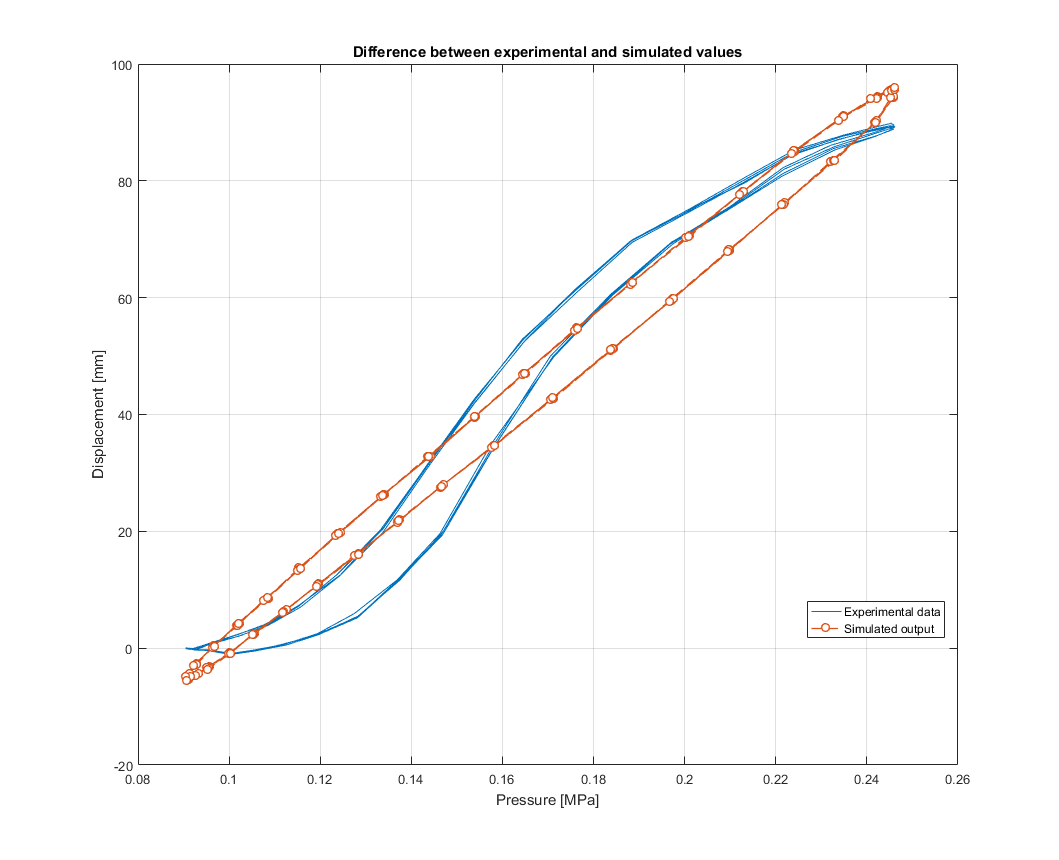
\includegraphics[width=\linewidth]{Images/comparison}
	\caption[Comparison between experimental data and simulated output]{Comparison between experimental data and simulated output}
	\label{fig:comparison}
\end{figure}

If the Bouc-Wen model is taken into consideration, then the parameters
must be fixed appropriately. To get a fairly good fit it is possible to tune
these parameters by trial and error. Further methods for finding the best sets
of parameters for the hysteresis model are discussed in Chapter~\ref{ch:optimization}.

\subsection{Classic Bouc-Wen Model Parameters}

\begin{minipage}{0.6\textwidth}
	\vspace*{-0.25cm}
	The parameters to be chosen for the classic version of the Bouc-Wen model are
	$\alpha$, $A$, $\beta$, $\gamma$ and $n$. For this work, $n$ will be fixed at 1
	for both the classic and generalized version of the hysteresis model.
	Details about how each parameters alters the shape of the hysteretic loop
	are in Appendix~\ref{app:bouc-wen}. 
	
	The parameters in Table~\ref{tab:classic_param} have been fixed by trial and error.
	All parameters are adimensional.	
\end{minipage}
\hfill
\begin{minipage}{0.35\textwidth}
	\vspace*{-0.5cm}
	\begin{table}[H]
		\centering
		\begin{tabular}{@{}cl@{}}
			\toprule
			\textbf{Parameter} & \textbf{Value} \\ \midrule
			$\alpha$           & $0.5$          \\
			$A$                & $0.9$          \\
			$\beta$            & $0.002$        \\
			$\gamma$           & $-0.001$       \\
			$n$                & $1$            \\ \bottomrule
		\end{tabular}
		\caption{Parameters for the Classic Bouc-Wen Model}
		\label{tab:classic_param}
	\end{table}
\end{minipage}

\vspace*{0.5cm}

Given experimental input $p$, the simulated output of the system taking into consideration
the classic Bouc-Wen model of hysteresis is shown in Figure~\ref{fig:comp_classic}.

\begin{figure}[H]
	\centering
	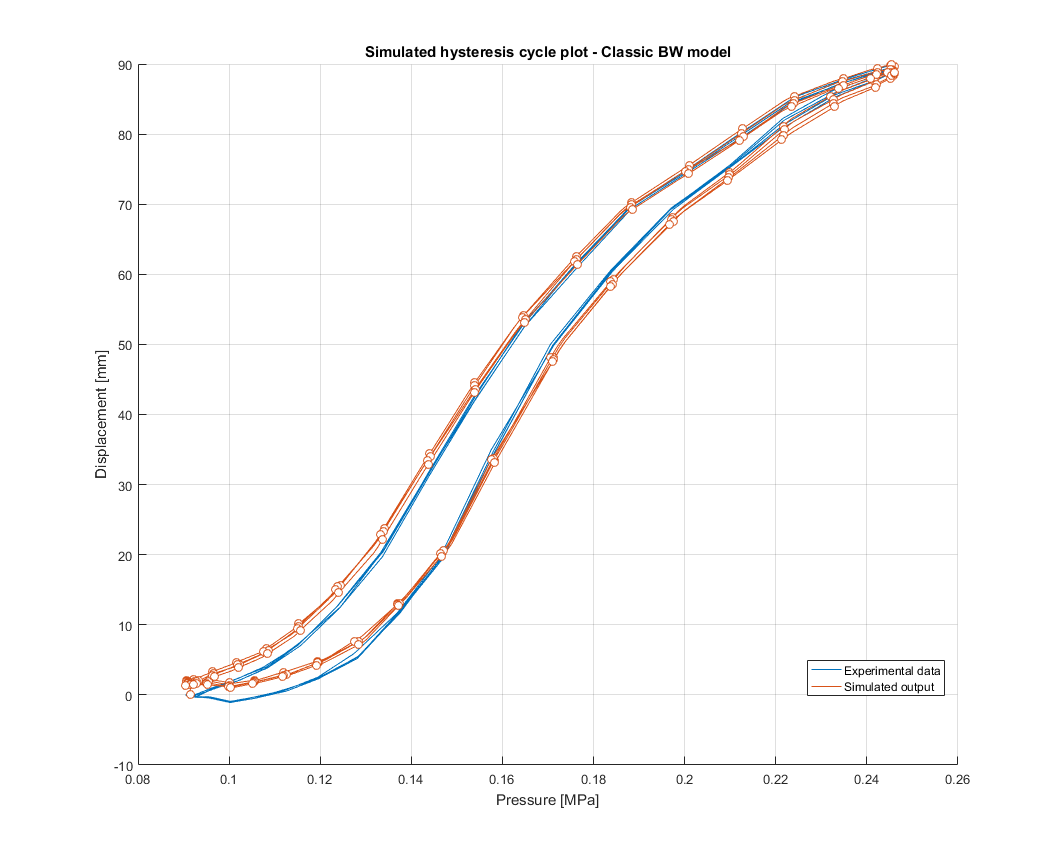
\includegraphics[width=\linewidth]{Images/comparison_classic}
	\caption[Comparison between experimental data and simulated output with classic Bouc-Wen model]{Comparison between experimental data and simulated output with classic Bouc-Wen model}
	\label{fig:comp_classic}
\end{figure}

\subsection{Generalized Bouc-Wen Model Parameters}

\begin{minipage}[ht]{0.6\textwidth}
	\vspace*{-2cm}
	The parameters to be chosen for the generalized version of the Bouc-Wen model
	are $\alpha$, $A$, $n$, $\beta_1$, \ldots, $\beta_6$. 
	As previously stated, the value of $n$ is fixed to $1$.
	
	As for the classic version of the hysteresis model, the parameters
	in Table~\ref{tab:gener_param} have been selected by trial and error.
	All parameters are adimensional.
	
	Given experimental input $p$, the simulated output of the system
	after taking into consideration the generalized Bouc-Wen model of hysteresis
	is shown in Figure~\ref{fig:comp_gener}.
\end{minipage}
\hfill
\begin{minipage}{0.35\textwidth}
	\vspace*{-0.5cm}
	\begin{table}[H]
		\centering
		\begin{tabular}{@{}cl@{}}
			\toprule
			\textbf{Parameter} & \textbf{Value} \\ \midrule
			$\alpha$           & $0.9$          \\
			$A$                & $1$          	\\
			$n$   		       & $1$        	\\
			$\beta_1$          & $0.01$       	\\
			$\beta_2$          & $0.005$       	\\
			$\beta_3$          & $0.1$       	\\
			$\beta_4$          & $-0.01$       	\\
			$\beta_5$          & $-0.1$       	\\
			$\beta_6$          & $0.001$       	\\ \bottomrule
		\end{tabular}
		\caption{Parameters for the Generalized Bouc-Wen Model}
		\label{tab:gener_param}
	\end{table}
\end{minipage}

\begin{figure}[H]
	\centering
	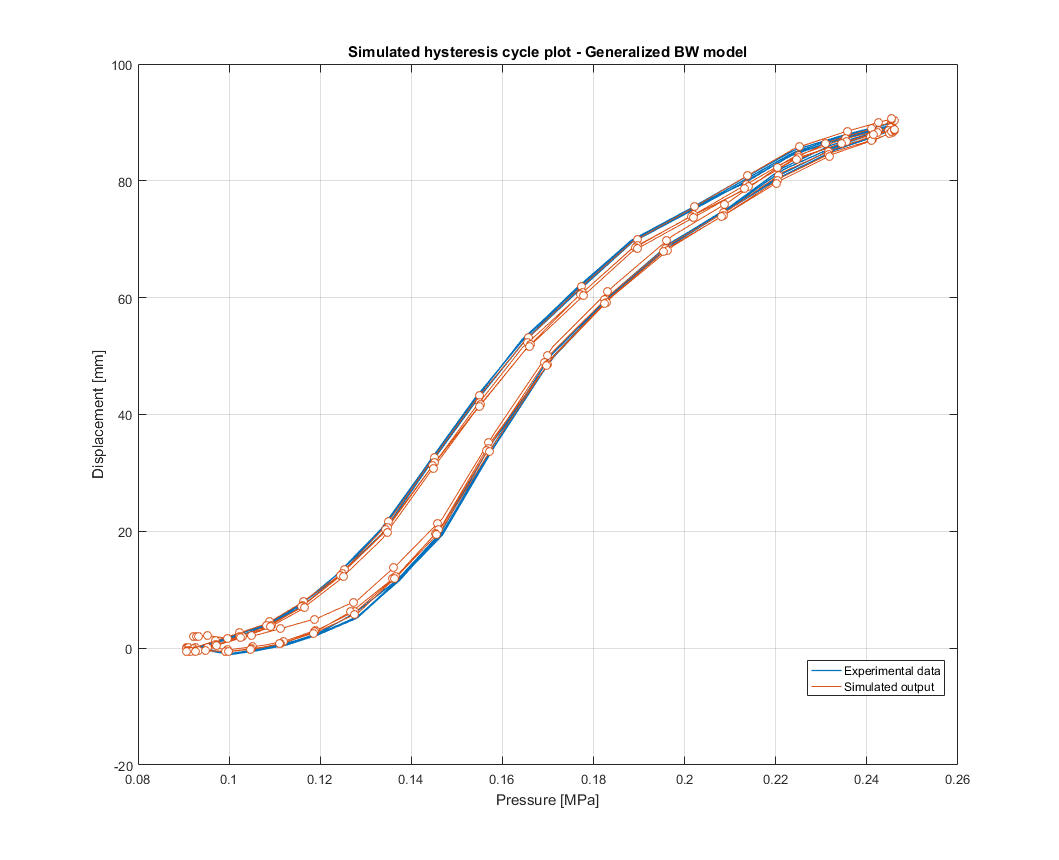
\includegraphics[width=\linewidth]{Images/comparison_general}
	\caption{Comparison between experimental data and simulated output with generalized Bouc-Wen model}
	\label{fig:comp_gener}
\end{figure}
